\begin{example}
    [While Odds Algorithm]
    \label{ex:whileOdd}
    { \small
    \begin{figure}
    \centering
    \begin{subfigure}{.4\textwidth}
      \begin{centering}
      {\small
      $
      \begin{array}{l}
        \kw{whileOdd}(k) \triangleq \\
        \clabel{ \assign{i}{k} }^{0} ; \\
            \ewhile ~ \clabel{i > 0}^{1} ~ \edo ~ \\
            \qquad \Big(
              \eif(\clabel{i \% 2 == 0 }^{2}, \\
              \qquad \qquad \clabel{\assign{i}{i - 1}}^{3},\\
              \qquad \qquad \clabel{\assign{i}{i - 3}}^{4});
              \Big)
        \end{array}
      $
      }
      \caption{}
      \end{centering}
      \end{subfigure}
    \begin{subfigure}{.5\textwidth}
      \begin{centering}
    %   \todo{abstract-cfg for two round}
    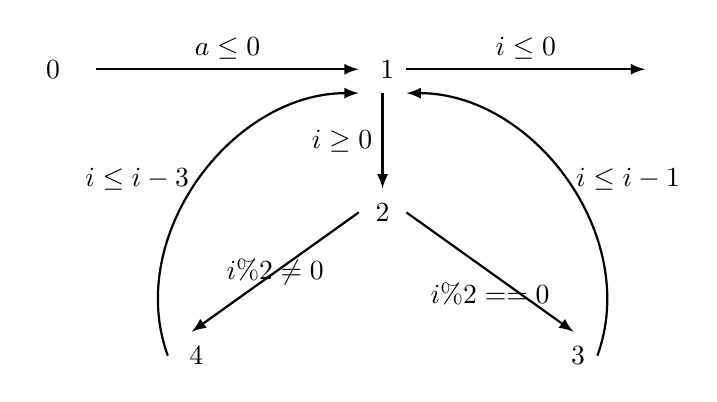
\begin{tikzpicture}[scale=\textwidth/20cm,samples=200]
    \draw[] (-7, 10) circle (0pt) node{{ $0$}};
    \draw[] (0, 10) circle (0pt) node{{ $1$}};
    \draw[] (0, 7) circle (0pt) node{\textbf{$2$}};
    \draw[] (4, 4) circle (0pt) node{{ $3$}};
    % \draw[] (0, 1) circle (0pt) node{{ $4$}};
    \draw[] (-4, 4) circle (0pt) node{{ $4$}};
    % Counter Variables
    \draw[] (6, 10) circle (0pt) node {\textbf{$\lex$}};
    % \draw[] (6, 4) circle (0pt) node {{ $ex$}};
    %
    % Control Flow Edges:
    \draw[ thick, -latex] (-6, 10)  -- node [above] {$a \leq 0$}(-0.5, 10);
    \draw[ thick, -latex] (0, 9.5)  -- node [left] {$i \geq 0$} (0, 7.5) ;
    \draw[ thick, -latex] (0.5, 7)  -- node [below] {$ i \% 2 == 0 $}  (4, 4.5);
    \draw[ thick, -latex] (-4.5, 4)  to  [out=110,in=180]  node [left] {$i \leq i - 3$ }(-0.5, 9.5);
    \draw[ thick, -latex] (4.5, 4)  to  [out=70,in=0]   node [right] {$i \leq i - 1$ }(0.5, 9.5);
    \draw[ thick, -latex]  (-0.5, 7) -- node  {$i \% 2 \neq 0$}  (-4, 4.5) ;
    \draw[ thick, -latex] (0.5, 10)  -- node [above] {$i \leq 0$}  (5.5, 10);
    % \draw[ thick, -latex] (6, 6.5)  -- node [right] {$\top$} (6, 4.5) ;
    \end{tikzpicture}
    \caption{}
      \end{centering}
      \end{subfigure}
    \caption{
    (a) The Simple While Loop Example with Two Paths
      (b) The Abstract Execution Control Flow Graph}
        \label{fig:whileOdd}
    \end{figure}
    }
    %
    \end{example}    
    \begin{enumerate}
      \item  \textbf{The Abstract Execution Control Flow Graph} is generated in Figure~\ref{fig:whileOdd}(b).
      Each directed edge represents a transition from the first control location to the next control location.
      Every edge is annotated by a constraint, such that the transition between the control locations satisfies.
    
    \item Program Rephrase and refinement. 
    \\
    The loop free transition paths are collected as follows,
    \[
      \begin{array}{ll}
        \tpath_0 = (0 \to 1)
        &
        \tpath_1 = (1 \to 2), (2 \to 3), (3 \to 1)
        \\
        \tpath_2 = (1 \to 2), (2 \to 4), (4 \to 1)
        &
        \tpath_3 = (1 \to \lex)
      \end{array}
      \]
    \textbf{Rephrased Program}:
    \[
    \tpath_0 ; LOOP1: \rprepeat(\rpchoose\{\tpath_1, \tpath_2 \}); \tpath_3
    \]
    \textbf{Refined Program}:
    \[
      \tpath_0 ; LOOP1: \rpchoose\{\rprepeat_3(\rprepeat_1(\tpath_1); \tpath_2) , \rprepeat_4(\rprepeat_2(\tpath_2); \tpath_1) \}; \tpath_3
      \]
    \item \textbf{Outside-In Algorithm} : Compute Local Bound for Every program and sub programs.
    \[
      \begin{array}{lll}
        LB(\tpath_0) = 1
        &
        LB(\tpath_3) = 1
        &
        LB(\rprepeat_3(\rprepeat_1(\tpath_1); \tpath_2)) = \frac{n}{4} 
        \\
        LB(\rprepeat_1(\tpath_1)) = 1 
        &
        LB(\rprepeat_2(\tpath_2)) = 1 
        &
        LB(\rprepeat_4(\rprepeat_2(\tpath_2); \tpath_1)) = \frac{n}{4}
      \end{array}
      \]
    %       $LB(\tpath_0) = 1$
    % \\
    % $LB(\tpath_3) = 1$
    % \\
    % $LB(\rprepeat_1(\tpath_1)) = 1 $
    % \\
    % $LB(\rprepeat_3(\rprepeat_1(\tpath_1); \tpath_2)) = \frac{n}{4} $
    % \\
    % $LB(\rprepeat_2(\tpath_2)) = 1 $
    % \\
    % $LB(\rprepeat_4(\rprepeat_2(\tpath_2); \tpath_1)) = \frac{n}{4} $
    % \\
    % $LB(LOOP1: \rpchoose(\rprepeat_2(\cdots), \rprepeat_1(\tpath_1))) 
    % = \max\{m, \frac{n}{m}\} $
    % \\
    \item \textbf{Inside-Out Algorithm}
    \begin{itemize}
      \item \textbf{Repeat Chain Set}
      \\
      $rp\mathcal{C}(LOOP1, \tpath_1) = \{\rprepeat_4(\cdots, \tpath_1), \rprepeat_3(\rprepeat_1(\tpath_1); \tpath_2) \to \rprepeat_1(\tpath_1)\}$ \\
      $rp\mathcal{C}(LOOP1, \tpath_2) = \{\rprepeat_3(\cdots, \tpath_2), \rprepeat_4(\rprepeat_2(\tpath_2); \tpath_1) \to \rprepeat_2(\tpath_2)\}$ \\
      $rp\mathcal{C}(\_, \_) = \emptyset$ 
      % \\
      \item \textbf{{Local Repeat Chain Bound} }for Every Transition Path $\tpath$ on its Repeat Chain
      $rpLB(LOOP1, \tpath_1) = \frac{n}{4}$ \\
      $rpLB(LOOP1, \tpath_2) = \frac{n}{4}$ 
      %
      \item \textbf{Loop Chain}
      \[
        \begin{array}{ll}
          lp\mathcal{C}(\tpath_1) = \{LOOP1\to \tpath_1\}
          &
          lp\mathcal{C}(\tpath_2) = \{LOOP1\to \tpath_2\}
          \\
          lp\mathcal{C}(\tpath_0) = \{\tpath_0\}
          &
          lp\mathcal{C}(\tpath_3) = \{\tpath_3\}
        \end{array}
        \]
      % $lp\mathcal{C}(\tpath_1) = \{LOOP1\to \tpath_1\}$ \\
      % $lp\mathcal{C}(\tpath_2) = \{LOOP1\to \tpath_2\}$ \\
      % $lp\mathcal{C}(\tpath_0) = \{\tpath_0\}$ \\
      % $lp\mathcal{C}(\tpath_3) = \{\tpath_3\}$ 
      \item \textbf{Nested Loop Bound }for Every Transition Path $\tpath$ on its Loop Chain
      \[
        \begin{array}{ll}
          rpLB(LOOP1, \tpath_1) = \frac{n}{4}
          &
          rpLB(LOOP1, \tpath_2) = \frac{n}{4}
          \\
          rpLB(\bot, \tpath_0) = 1
          &
          rpLB(\bot, \tpath_3) = 1
        \end{array}
        \]
      % $rpLB(LOOP1, \tpath_1) = \frac{n}{4}$ \\
      % $rpLB(LOOP1, \tpath_2) = \frac{n}{4}$  \\
      % $rpLB(\bot, \tpath_0) = 1$ \\
      % $rpLB(\bot, \tpath_3) = 1$ 
      \item \textbf{Path Sensitive Reachability Bound} For Every Transition Path $\tpath$ 
      \\
      $psRB(\tpath_1) = \frac{n}{4}$ \quad
      $psRB(\tpath_2) = \frac{n}{4}$ \quad
      $psRB(\tpath_0) = 1$ \quad
      $psRB(\tpath_3) = 1$ 
    \end{itemize}
    \item \textbf{Path Sensitive Reachability Bound} Computation for Every Location
    \\
    $psRB(\{0, 1\}) = 1$ \quad
    $psRB(\{2, 3, 1 \}) = \frac{n}{4}$ \quad
    $psRB(\{2, 4, 1\}) = \frac{n}{4}$ \quad
    $psRB(\{\lex\}) = 1$ 
    \end{enumerate}

